% NOTE: source arXiv 2505.22954 presents this figure and
% figures/04_dgm_progress.tex side by side in one combined float with two
% \label commands (fig:dgm-archive, fig:dgm-progress) both pointing at the
% same figure number; both labels are independently \Cref'd elsewhere in the
% paper. Split into two single-asset floats to satisfy
% paper/figures/README.md's one-wrapper-per-one-asset convention. See
% paper/supplementary/source-attribution.md.
\begin{figure}[ht]
\centering
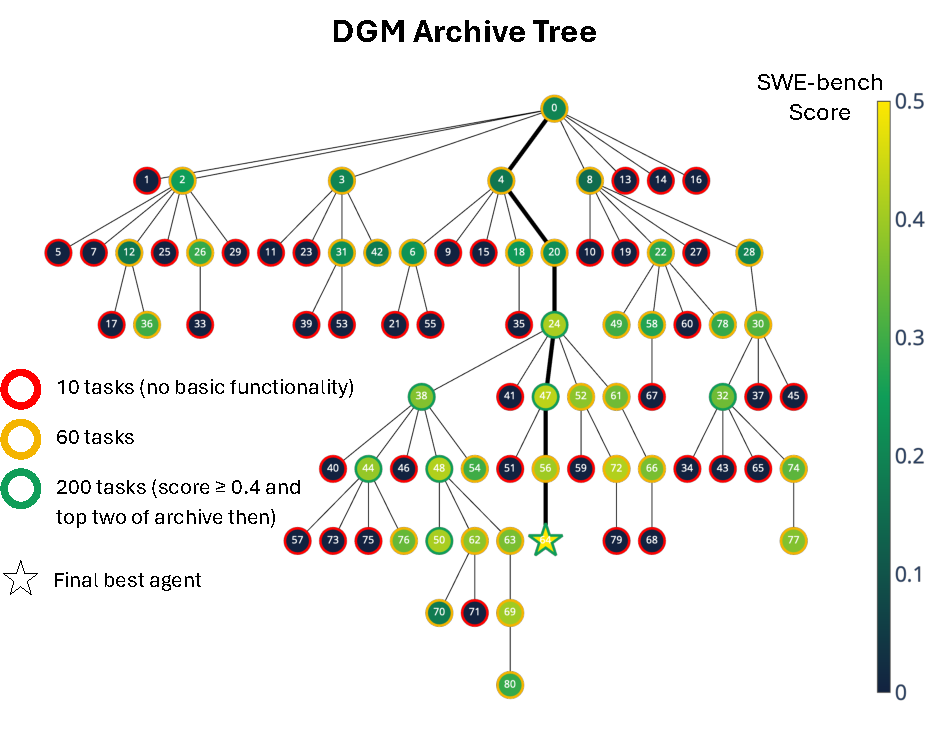
\includegraphics[width=0.9\textwidth]{figures/srcs/03_dgm_archive.pdf}
\caption{\textbf{The DGM automatically self-improves to become a better coding agent.} (Left) Archive of coding agents generated during the DGM run on SWE-bench. Each node represents a coding agent, with node 0 corresponding to the base agent. Node color indicates performance on SWE-bench (percentage of solved tasks), while border color reflects the number of tasks for which the agent was evaluated. Edges show which agents self-modified to produce the offsprings. Many paths to innovation traverse lower-performing nodes, and key innovations (like node 24) lead to an explosion of innovations built on top of them. Both properties underscore the benefits of open-ended search. (Right) Progress plot of the DGM on SWE-bench, see \Cref{fig:dgm-progress}.}
\label{fig:dgm-archive}
\end{figure}
